\section{Accuracy improvement with newly fitted acceptance policies}
\label{app:accuracy}
\subsection{A distinct retrospective protocol}
The additional experiment uses only the 1,829 development items and origin-valid observations; neither historical holdout is accessed. All dates have been consumed in prior research. A protocol records the predictor identities, chronological blocks, head specification, utility grid, cap, floor, and bootstrap before the additional head fits. This order makes the computation auditable; it does not erase previous knowledge of evaluation performance.

The group-scaled predictor is the first hierarchy-feature XGBoost L1 fit from the forecasting experiments, trained on observed sales with 33 origin-valid features and seven cross-store item summaries. A separately learned observable capacity-hit probability $q$ is available. The residual predictor is
\[
 f_{\rm res}(X)=\max\{f_0(X)+g(X,f_0(X),q(X)),0\},
\]
where $g$ is L1 gradient boosting trained on retained-target residuals. Days 1314--1373 fit candidate corrections and 1374--1433 select depth in $\{2,4\}$ and tree count in $\{50,150,300\}$; parent scaling is a fallback. Learning rate is 0.03 and minimum leaf sample size is 50. The selected depth-4, 300-tree correction is refitted on their union (up to 400,000 sampled rows). No accuracy parameter is retuned during the new selector comparison. The correction is conventional residual learning, not a proposed architecture.

Chronos-2 uses the archived univariate, nonnegative median forecasts, context up to 2,048, horizon seven, and no cross-series learning. Weight revision, weight hashes, and prediction receipts accompany the data. Raw backbone outputs are used; the older risk-bin recalibration, which was fitted on an overlapping block, is deliberately not used in this comparison. Foundation pretraining and task-specific supervised forecasting have different information histories; the within-predictor utility contrasts are the target.

The new demand head sees 40 history/hierarchy features and $q$. Each predictor-specific error head also sees that predictor's forecast. Heads use squared loss, 220 trees, 31 leaves, learning rate 0.05, minimum leaf size 50, deterministic four-thread fitting, and seed 20260908. The same 600,000 sampled training rows supply $Y$ to the demand head and $|Y-f|$ to each error head. Both outputs are clipped to nonnegative values. Thus the acceptance experiment intentionally uses benchmark truth labels; it is not an observed-sales-only solution for naturally hidden demand.

The earliest calibration origin is 1610, after all head-training targets through 1610 have been observed. The two blocks contain 35 and 28 target days; evaluation contains 114 target days with origins at least 1799. The training sample's mean demand estimates $T$. For each $\lambda\in\{1,0.25,0\}$, all distinct finite score thresholds are searched, whole ties are retained, and the largest threshold meeting pooled WAPE and row-floor constraints in both blocks is fixed. No test outcome selects a threshold or utility weight. An infeasible search would return full abstention; all nine searches are feasible. The cap uses the displayed reference $0.85\times0.7530939208$, differing from the historical full-precision cap by less than $3\times10^{-11}$.

\begin{table}[htbp]\centering\small
\caption{New within-predictor contrasts versus $\lambda=1$, in percentage points. Marginal 95\% paired item-bootstrap intervals condition on the fits and research history; 4,000 draws, 1,829 items. The pure-demand endpoint $\lambda=0$ is included without a denominator floor.}
\label{tab:accuracy-ci}
\begin{tabular}{lrrrrr}\toprule
Predictor & $\lambda$ & $\Delta$ rows & Interval & $\Delta$ demand & Interval\\\midrule
Group-scaled L1 & 0.25 & -5.77 & $[-6.45,-5.05]$ & +5.47 & $[4.34,6.64]$ \\
Group-scaled L1 & 0 & -24.07 & $[-25.50,-22.62]$ & +6.70 & $[4.92,8.53]$ \\
Residual L1 & 0.25 & -3.02 & $[-3.57,-2.43]$ & +5.87 & $[4.84,6.88]$ \\
Residual L1 & 0 & -16.87 & $[-18.07,-15.61]$ & +7.36 & $[5.78,8.94]$ \\
Chronos-2 (raw) & 0.25 & -5.35 & $[-5.96,-4.69]$ & +6.39 & $[5.45,7.31]$ \\
Chronos-2 (raw) & 0 & -22.95 & $[-24.38,-21.50]$ & +8.18 & $[6.74,9.60]$ \\\bottomrule\end{tabular}\end{table}
\begin{table}[htbp]\centering\small
\caption{Calibration pooled and later category WAPE for the new predictors. The cap is 0.64013. All nine policies meet both calibration point constraints; Hobbies and Household miss the later cap.}
\label{tab:accuracy-groups}
\begin{tabular}{lrrrrr}\toprule
Predictor & $\lambda$ & Cal. A/B & Foods & Hobbies & Household\\\midrule
Group-scaled L1 & 1 & 0.6401/0.6259 & 0.5902 & 0.8468 & 0.6839 \\
Group-scaled L1 & 0.25 & 0.6401/0.6228 & 0.5903 & 0.8321 & 0.6753 \\
Group-scaled L1 & 0 & 0.6401/0.6215 & 0.5966 & 0.8135 & 0.6612 \\
Residual L1 & 1 & 0.6401/0.6252 & 0.5901 & 0.8518 & 0.6855 \\
Residual L1 & 0.25 & 0.6401/0.6232 & 0.5894 & 0.8366 & 0.6785 \\
Residual L1 & 0 & 0.6401/0.6233 & 0.5940 & 0.8295 & 0.6699 \\
Chronos-2 (raw) & 1 & 0.6401/0.6301 & 0.5909 & 0.8520 & 0.6870 \\
Chronos-2 (raw) & 0.25 & 0.6401/0.6259 & 0.5898 & 0.8354 & 0.6744 \\
Chronos-2 (raw) & 0 & 0.6401/0.6251 & 0.5967 & 0.8164 & 0.6603 \\\bottomrule\end{tabular}\end{table}
\begin{table}[htbp]\centering\small
\caption{Budget decomposition for $\lambda=1$ versus $\lambda=0.25$ in the new retrospective comparison. Demand share uses the whole evaluation denominator; excess is absolute-error mass minus $r$ times demand mass. Negative common excess supplies slack.}
\label{tab:accuracy-budget}
\begin{tabular}{llrrrrr}\toprule
Predictor & Set & Rows & Demand (\%) & WAPE & Mean $f$ & Excess\\\midrule
Group-scaled L1 & Common & 1,594,575 & 77.24 & 0.6169 & 1.018 & -52,237.9 \\
Group-scaled L1 & Row only & 196,485 & 3.35 & 0.9966 & 0.076 & 34,812.8 \\
Group-scaled L1 & Mixed only & 76,262 & 8.82 & 0.7481 & 1.988 & 27,784.7 \\
Residual L1 & Common & 1,730,317 & 81.30 & 0.6218 & 0.977 & -43,525.8 \\
Residual L1 & Row only & 135,756 & 2.55 & 0.9904 & 0.107 & 26,046.8 \\
Residual L1 & Mixed only & 72,762 & 8.42 & 0.7217 & 2.208 & 20,039.0 \\
Chronos-2 (raw) & Common & 1,493,529 & 72.28 & 0.6196 & 0.955 & -43,234.8 \\
Chronos-2 (raw) & Row only & 190,032 & 3.14 & 1.0049 & 0.070 & 33,442.0 \\
Chronos-2 (raw) & Mixed only & 78,383 & 9.53 & 0.7092 & 2.115 & 19,221.3 \\\bottomrule\end{tabular}\end{table}
The paired bootstrap resamples 1,829 item clusters, retaining all stores and dates, with 4,000 draws at seed 20260908. These are marginal descriptive percentile intervals conditional on the predictors, fitted heads, chosen policies, and adaptive research history. They do not include model-fitting uncertainty or shared calendar/store shocks. Item sufficient statistics reproduce all intervals; saved forecast and head arrays reproduce masks and budget sums.

\subsection{Coverage results for the three archived predictors}
\label{sec:accuracy}
Better forecasts can expand useful acceptance, but this alone does not specify how to spend the error budget. If a predictor's full-coverage risk is at most $r$, accepting all cases is a common optimum and mismatch disappears. Full-coverage risk above the cap is necessary for a strict objective reversal, but it is not sufficient: the same selective rule can still optimize both utilities (Appendix~\ref{app:necessity}). We test empirically whether reversal persists for the improved predictors here.

We use the three archived predictors and shared dates defined above in Appendix~\ref{app:accuracy}. Chronos-2 weights remain frozen \citep{ansari2025chronos2}; its selector is task-trained. This tests acceptance within each pipeline, not training-matched backbone superiority.

\begin{table}[H]
\centering\small
\caption{New retrospective comparison on the same 2,085,060 M5 development evaluation rows. Each predictor has a newly fitted error head; all share a newly fitted demand head, head-training rows, cap, and calibration dates. Higher coverage is better; lower WAPE is better. Full WAPE uses every row. These are fitted-policy outcomes, not population optima or a new external test.}
\label{tab:accuracy-selection}
\begin{tabular}{lrrrrr}\toprule
Predictor & Full WAPE & $\lambda$ & Rows (\%) & Demand (\%) & Accepted WAPE\\\midrule
Group-scaled L1 & 0.67139 & 1 & 85.90 & 80.59 & 0.63272 \\
Group-scaled L1 & 0.67139 & 0.25 & 80.13 & 86.06 & 0.63039 \\
Residual L1 & 0.65956 & 1 & 89.50 & 83.85 & 0.63298 \\
Residual L1 & 0.65956 & 0.25 & 86.48 & 89.72 & 0.63116 \\
Chronos-2 (raw) & 0.68310 & 1 & 80.74 & 75.42 & 0.63568 \\
Chronos-2 (raw) & 0.68310 & 0.25 & 75.39 & 81.82 & 0.63007 \\
\bottomrule\end{tabular}
\end{table}

The residual learner lowers full-coverage WAPE by 1.76\% relative to category-scaled L1. Both its row-weighted and mixed policies increase \emph{both} coverages over the corresponding base policies. Yet switching utility within that improved predictor still gains 5.87 demand-coverage points while losing 3.02 row points. The paired item-bootstrap intervals are $[4.84,6.88]$ and $[-3.57,-2.43]$ points, respectively. The same signs occur for the base and Chronos predictors, and for all three pure-demand endpoints (Appendix Table~\ref{tab:accuracy-ci}). These are retrospective, fit-conditional comparisons.

\begin{figure}[t]
\centering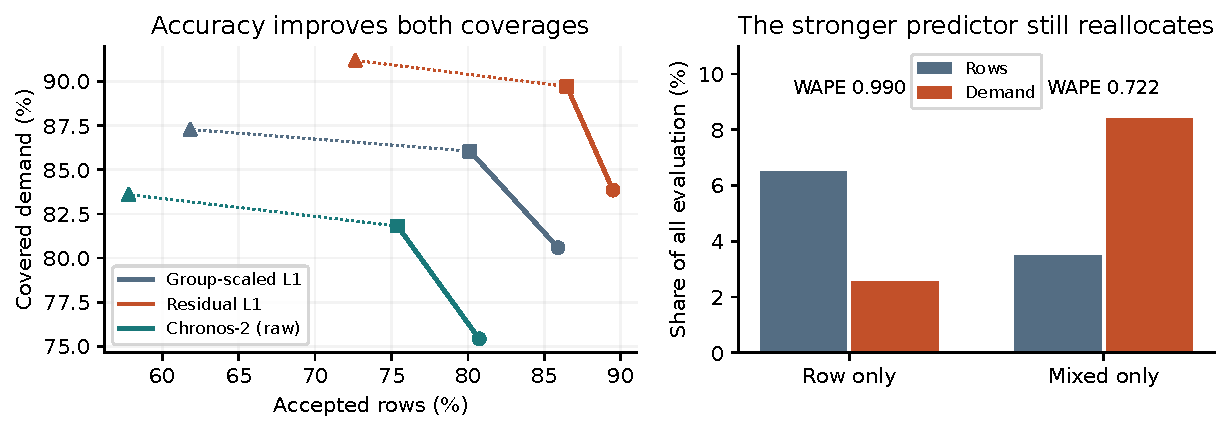
\includegraphics[width=\linewidth]{figures/accuracy_coverage.pdf}
\caption{Matched-date comparison. Left: moving to a stronger predictor raises both coverages, while changing utility within a predictor trades them off. Circles, squares, and triangles denote $\lambda=1,0.25,0$. Lines connect evaluated settings, not Pareto frontiers. Right: the improved predictor's exclusive acceptance sets retain the budget mechanism.}
\label{fig:accuracy}
\end{figure}
The improved mixed policy also exceeds the base row policy in both coverages (86.48/89.72 versus 85.90/80.59 percent). Nevertheless, its row-only set carries just 2.55\% of demand while spending 59.84\% of common slack (Appendix~\ref{app:accuracy}). The smaller case sacrifice (3.02 versus 5.77 points) coexists with the same mechanism. Neither pooled policy establishes the Hobbies or Household cap.


\subsection{What the additional forecasting controls establish}
The preceding forecasting study includes fixed risk-bin recalibration, forecast-value bins, top-risk-only uplift, minimum-support fallback, separately tuned residual learning with and without $q$, and frozen-backbone recalibration. Its role here is to supply stronger predictors and explicit limits on interpretation, not to claim a universally superior risk coordinate.

\begin{table}[htbp]\centering\small
\caption{Retained forecasting controls. All later learned-model comparisons are retrospective. FreshRetailNet non-stockout rows condition on realized availability; all-row metrics target recorded sales, not latent demand. M5 is the first-seed later development block.}
\label{tab:forecast-controls}
\begin{tabular}{lrrr}\toprule
Forecast & M5 & FRN non-stockout & FRN all sales\\\midrule
Group scale & 0.67139 & 0.32928 & 0.36162\\
Forecast-value bins & 0.67045 & 0.32753 & 0.36154\\
Risk bins & 0.66851 & 0.32741 & 0.36033\\
Top-risk-only uplift & 0.66843 & 0.32504 & 0.35938\\
Residual L1 with $q$ & 0.65956 & 0.29201 & 0.33401\\
Residual L1 without $q$ & 0.66532 & 0.29289 & 0.33463\\\bottomrule
\end{tabular}\end{table}

On M5, bin-based recalibration adds only a modest gain over the parent and does not beat the residual learner. On FreshRetailNet, a 2,000-series cohort was fixed from training data before the original one-time seven-day evaluation. Its original risk-bin versus parent comparison has uncertainty sensitive to clustering. Later forecast-bin, uplift, and learned controls reuse this cohort; they are not additional prospective tests. The original non-stockout population contains 8,020 rows, versus 14,000 recorded-sales rows overall. Training/selection for the residual learner uses the chronological tail of the training partition (earlier two blocks for fitting; later three for selection), then refits on all five. The same six-setting grid selects depth 4 and 300 trees. The base, risk head, and categorical encoder remain fixed from earlier training.

FreshRetailNet risk-bin minus residual WAPE is 0.03541 on non-stockout rows. Paired 95\% intervals are [0.02813,0.04273] by series, [0.02824,0.04368] by store, [0.01535,0.05326] by product, and [0.02135,0.04983] by date; only seven dates are available. The no-$q$ follow-up is adaptive and separately tuned. Its WAPE difference from the full residual learner is 0.00088, with product-cluster interval [$-0.00016$,0.00197]. Most forecasting improvement therefore cannot be attributed to the risk feature. The corrected predictor's RMSE decreases from 0.74595 to 0.62157 and signed bias from $-14.04\%$ to $-1.92\%$ on that population. It still worsens 777 of 2,000 series. None of these observations identifies demand on stockout rows or measures inventory cost.

Frozen Chronos recalibration also improves within-backbone WAPE, but its calibration period differs from that of the main tabular predictor and its bin-control advantage changes under asymmetric pinball losses. These historical comparisons are preserved in the forecasting evidence archive. They are not pooled with the original external test or counted as independent natural-demand confirmation. Numerical dependency repairs and column-label audits are recorded there; the selected forecasts used in the present experiment reproduce the corrected reference values exactly.
